\chapter{Implementación}
Durante la implementación, se ha seguido la planificación y metodologías
anteriormente descritas, dividiendo el proyecto en tareas más pequeñas y
manejables, para que se puedan realizar en un periodo de tiempo razonable.

Al seguir la prioridad de las tareas, se realizan primero las tareas más
críticas, como la creación de la infraestructura y la ingesta de las fuentes
esenciales, y se dejan para más adelante tareas como la visualización para
clientes externos o fuentes menos críticas y más complejas, como las APIs de
terceros o el \textit{web scraping}.


\section{Despliegue local}\label{sec:impl_local}
Para arrancar el desarrollo del proyecto, se implementa una versión local del
sistema, que permita trabajar en un entorno controlado y sin dependencias
externas para comprobar su correcto funcionamiento y establecer
las configuración base para su posterior despliegue en la nube.

Puesto que se ha decidido utilizar Docker para la gestión de contenedores, se
crea un archivo \texttt{docker-compose.yml} que define los servicios
necesarios para el proyecto, es decir, \textit{Kafka}, \textit{Zookeeper},
\textit{Elasticsearch}, \textit{Kibana} y \textit{Logstash}, ignorando por
el momento la ingesta de datos y la escalabilidad del sistema.

Para la configuración de los servicios, se ha creado un archivo \texttt{.env}
que define las variables de entorno necesarias para el correcto funcionamiento
de los servicios, como las contraseñas o la versión del \textit{stack}.

Esta sección de la documentación documenta el desarrollo de la historia de
usuario inicial, de acuerdo con lo establecido en la sección \fullref{sec:planif_inicial}:

\begin{table}[H]
	\centering
	\begin{tabular}{|p{0.7\linewidth}|c|c|}
		\hline
		\textbf{Nombre} & \textbf{Prioridad} & \textbf{Tamaño} \\
		\hline
		\hline
		Creación de la infraestructura base (técnica) & P0\cellcolor{red!50} & L\cellcolor{orange!50} \\
		\hline
  	\end{tabular}
  	\caption{Lista de HUs cumplimentadas con el despliegue local}
  	\label{tab:impl_local}
\end{table}


\newpage{}
\subsection{Explicación del código}
\emph{El código de despliegue local se encuentra en el anexo \fullref{anexo:local}.}

A nivel de configuración, se definen variables de entorno para cada contenedor
mediante el uso de la palabra clave \texttt{environment} y las claves definidas
por cada imagen. Para cada contenedor, se define además información adicional
dependiendo de las características del servicio, como la dependencia en otras
imágenes, los límites de recursos o los puertos de escucha.

Para evitar el ruido excesivo por consola una vez arrancado los servicios, se
reduce el nivel de \textit{logging} a \textit{WARN} en los servicios que lo
soporten.

Durante el arranque de los contenedores, se ejecuta un script de inicialización
que se encarga de crear las credenciales y los usuarios necesarios para el
funcionamiento de los servicios. Estas credenciales son necesarias ya que los
contenedores funcionan mediante tráfico HTTPS.

Los contenedores cuentan con comprobaciones de salud (o \textit{health-checks})
básicas para asegurar que los servicios se han arrancado correctamente y están
funcionando.

Al comienzo del archivo \texttt{docker-compose.yml}, se definen los volúmenes y
las redes necesarias para el correcto funcionamiento de los servicios.

\begin{lstlisting}[style=yaml, caption={Definición de volúmenes y redes en Docker Compose}]
volumes:
	es01data:
	kibanadata:
	elasticdata:
	logstashdata:
	kafkadata:
	certs:

networks:
	default:
		driver: bridge
\end{lstlisting}

A continuación, se definen los servicios necesarios para el proyecto, comenzando
por el contenedor de preparación de credenciales y usuarios. Se utiliza una
imagen de Elasticsearch para la creación de las credenciales, y se monta un
volumen para la persistencia de las mismas.

\begin{lstlisting}[style=yaml, caption={Definición del servicio de preparación}]
setup:
  image: docker.elastic.co/elasticsearch/elasticsearch:${STACK_VERSION}
  volumes:
    - certs:/usr/share/elasticsearch/config/certs
    - ./setup.sh:/usr/local/bin/setup.sh
  user: root
  container_name: setup
  command: ["/bin/bash", "/usr/local/bin/setup.sh"]
  healthcheck:
    test: [ "CMD-SHELL", "[ -f config/certs/es01/es01.crt ]" ]
    interval: 5s
    timeout: 10s
    retries: 10
\end{lstlisting}

El servicio de preparación necesita tener una comprobación de salud, puesto que
el resto de contenedores lo tienen marcado como dependencia para su arranque. En
este caso, la comprobación consiste en la existencia de un archivo de
certificado.

Una vez definido el servicio de preparación, se definen los servicios de
\textit{Kafka} y \textit{Zookeeper}, que se basan en imágenes oficiales de
\textit{Confluent}.

\begin{lstlisting}[style=yaml, caption={Definición de los servicios de Kafka}]
zookeeper:
	container_name: zookeeper
	image: confluentinc/cp-zookeeper:latest
	environment:
	ZOOKEEPER_CLIENT_PORT: 2181
	ZOOKEEPER_TICK_TIME: 2000
	ZOO_LOG4J_PROP: WARN,CONSOLE
	ports:
	- 2181:2181

kafka:
	container_name: kafka
	image: confluentinc/cp-kafka:latest
	depends_on:
		- zookeeper
		- es01
	ports:
		- 9092:9092
		- 29092:29092
	environment:
		KAFKA_BROKER_ID: 1
		KAFKA_ZOOKEEPER_CONNECT: zookeeper:2181
		KAFKA_ADVERTISED_LISTENERS: LISTENER_DOCKER_INTERNAL://kafka:29092,LISTENER_DOCKER_EXTERNAL://localhost:9092
		KAFKA_LISTENER_SECURITY_PROTOCOL_MAP: LISTENER_DOCKER_INTERNAL:PLAINTEXT,LISTENER_DOCKER_EXTERNAL:PLAINTEXT
		KAFKA_INTER_BROKER_LISTENER_NAME: LISTENER_DOCKER_INTERNAL
		KAFKA_OFFSETS_TOPIC_REPLICATION_FACTOR: 1
		KAFKA_LOG4J_ROOT_LOGLEVEL: WARN
		KAFKA_TOOLS_LOG4J_LOGLEVEL: ERROR
		KAFKA_LOG4J_LOGGERS: 'kafka=WARN,kafka.controller=WARN,kafka.log.LogCleaner=WARN,state.change.logger=WARN,kafka.producer.async.DefaultEventHandler=WARN'
\end{lstlisting}

Ambos servicios cuentan con una serie de variables de entorno que definen su
configuración, como el puerto de escucha, el \textit{broker ID} o la dirección
de \textit{Zookeeper}.

Una vez definidos los servicios de Kafka, se define el servicio más crítico, el
contenedor de Elasticsearch, del que depende el funcionamiento de todo el
sistema.

\begin{lstlisting}[style=yaml, caption={Definición del servicio de Elasticsearch}]
es01:
    image: docker.elastic.co/elasticsearch/elasticsearch:${STACK_VERSION}
    container_name: es01
    restart: unless-stopped
    depends_on:
      - setup
    environment:
      - node.name=es01
      - cluster.name=${CLUSTER_NAME}
      - discovery.type=single-node
      - bootstrap.memory_lock=true
      - logger.level=WARN
      - ELASTIC_PASSWORD=${ELASTIC_PASSWORD}
      - xpack.security.enabled=true
      - xpack.security.http.ssl.enabled=true
      - xpack.security.http.ssl.key=certs/es01/es01.key
      - xpack.security.http.ssl.certificate=certs/es01/es01.crt
      - xpack.security.http.ssl.certificate_authorities=certs/ca/ca.crt
      - xpack.security.transport.ssl.enabled=true
      - xpack.security.transport.ssl.key=certs/es01/es01.key
      - xpack.security.transport.ssl.certificate=certs/es01/es01.crt
      - xpack.security.transport.ssl.certificate_authorities=certs/ca/ca.crt
      - xpack.security.transport.ssl.verification_mode=certificate
    ulimits:
      memlock:
        soft: -1
        hard: -1
      nofile:
        soft: 65536
        hard: 65536
    cap_add:
      - IPC_LOCK
    labels:
      co.elastic.logs/module: elasticsearch
      co.elastic.metrics/module: elasticsearch
    volumes:
      - es01data:/usr/share/elasticsearch/data
      - certs:/usr/share/elasticsearch/config/certs
    ports:
      - 9200:9200
    healthcheck:
      test:
        [
          "CMD-SHELL",
          "curl -s --cacert config/certs/ca/ca.crt https://localhost:9200 | grep -q 'missing authentication credentials'"
        ]
      interval: 10s
      timeout: 10s
      retries: 10
\end{lstlisting}

Debido a que se trata del servicio más importante y grande, se requieren muchas
opciones de configuración, como la limitación de recursos, la persistencia de
datos o la configuración de seguridad. Como en el resto de servicios, se define
una comprobación de salud que se encarga de comprobar que el servicio está
disponible.

Para simplificar lo máximo posible la arquitectura de este prototipo, tan solo
se define un nodo de Elasticsearch, aunque la configuración de escalabilidad
sería sencilla gracias al diseño de Docker.

Por último, se definen los servicios de Kibana y Logstash, que dependen de
Elastic.

\begin{lstlisting}[style=yaml, caption={Definición de los servicios de Kibana}]
kibana:
    container_name: kibana
    image: docker.elastic.co/kibana/kibana:${STACK_VERSION}
    restart: unless-stopped
    volumes:
      - kibanadata:/usr/share/kibana/data
      - certs:/usr/share/kibana/config/certs
    environment:
      SERVER_NAME: kibana
      SERVER_PORT: 5601
      SERVER_HOST: 0.0.0.0
      ELASTICSEARCH_HOSTS: https://es01:9200
      ELASTICSEARCH_USERNAME: kibana_system
      ELASTICSEARCH_PASSWORD: ${KIBANA_PASSWORD}
      ELASTICSEARCH_SSL_CERTIFICATEAUTHORITIES: config/certs/ca/ca.crt
      LOGGING_ROOT_LEVEL: warn
      XPACK_ENCRYPTEDSAVEDOBJECTS_ENCRYPTIONKEY: ${KEY}
      XPACK_REPORTING_ENCRYPTIONKEY: ${KEY}
      XPACK_SECURITY_ENCRYPTIONKEY: ${KEY}
    links:
      - es01
    depends_on:
      - setup
      - es01
    labels:
      co.elastic.logs/module: kibana
      co.elastic.metrics/module: kibana
    ports:
      - 5601:5601
    healthcheck:
      test:
        [
          "CMD-SHELL",
          "curl -s -I http://localhost:5601 | grep -q 'HTTP/1.1 302 Found'"
        ]
      interval: 10s
      timeout: 10s
      retries: 10
\end{lstlisting}

\begin{lstlisting}[style=yaml, caption={Definición de los servicios de Logstash}]
logstash:
  container_name: logstash
  image: docker.elastic.co/logstash/logstash:${STACK_VERSION}
  restart: unless-stopped
  user: root
  volumes:
    - logstash-data:/usr/share/logstash/data
    - certs:/usr/share/logstash/certs
    - ./logstash.conf:/usr/share/logstash/pipeline/logstash.conf
  environment:
    - ELASTIC_HOSTS=https://es01:9200
    - ELASTIC_USER=elastic
    - ELASTIC_PASSWORD=${ELASTIC_PASSWORD}
    - log.level=warn
    - xpack.monitoring.enabled=false
  command: bin/logstash -f /usr/share/logstash/pipeline/logstash.conf
  ports:
    - 5000:5000
  depends_on:
    - es01
    - kafka
    - setup
  labels:
    co.elastic.logs/module: logstash
    co.elastic.metrics/module: logstash
  links:
    - es01
    - kibana
\end{lstlisting}

Se hace uso de la red interna de Docker para facilitar la comunicación entre los
contenedores, y se definen comprobaciones de salud para asegurar que los
servicios se han arrancado correctamente. Para Logstash, se define un script de
lanzamiento que genera el archivo de configuración y ejecuta el servicio, aunque
podría montarse un volumen con el archivo de configuración ya generado.

\newpage{}
\subsection{Uso del sistema}
Una vez arrancados los contenedores mediante el comando
\texttt{docker compose up}, se puede acceder a los servicios a través de la
dirección local \texttt{localhost}. En el caso de Kibana, se puede acceder a
la interfaz de usuario mediante la dirección \texttt{localhost:5601}. En el
caso de Elasticsearch, se pueden hacer peticiones HTTPS a través de la dirección
\texttt{localhost:9200}. Para Kafka, Zookeeper y Logstash, se pueden hacer
peticiones a través de las direcciones \texttt{localhost:9092},
\texttt{localhost:2181} y \texttt{localhost:9600}, respectivamente.

\begin{figure}[H]
	\centering
	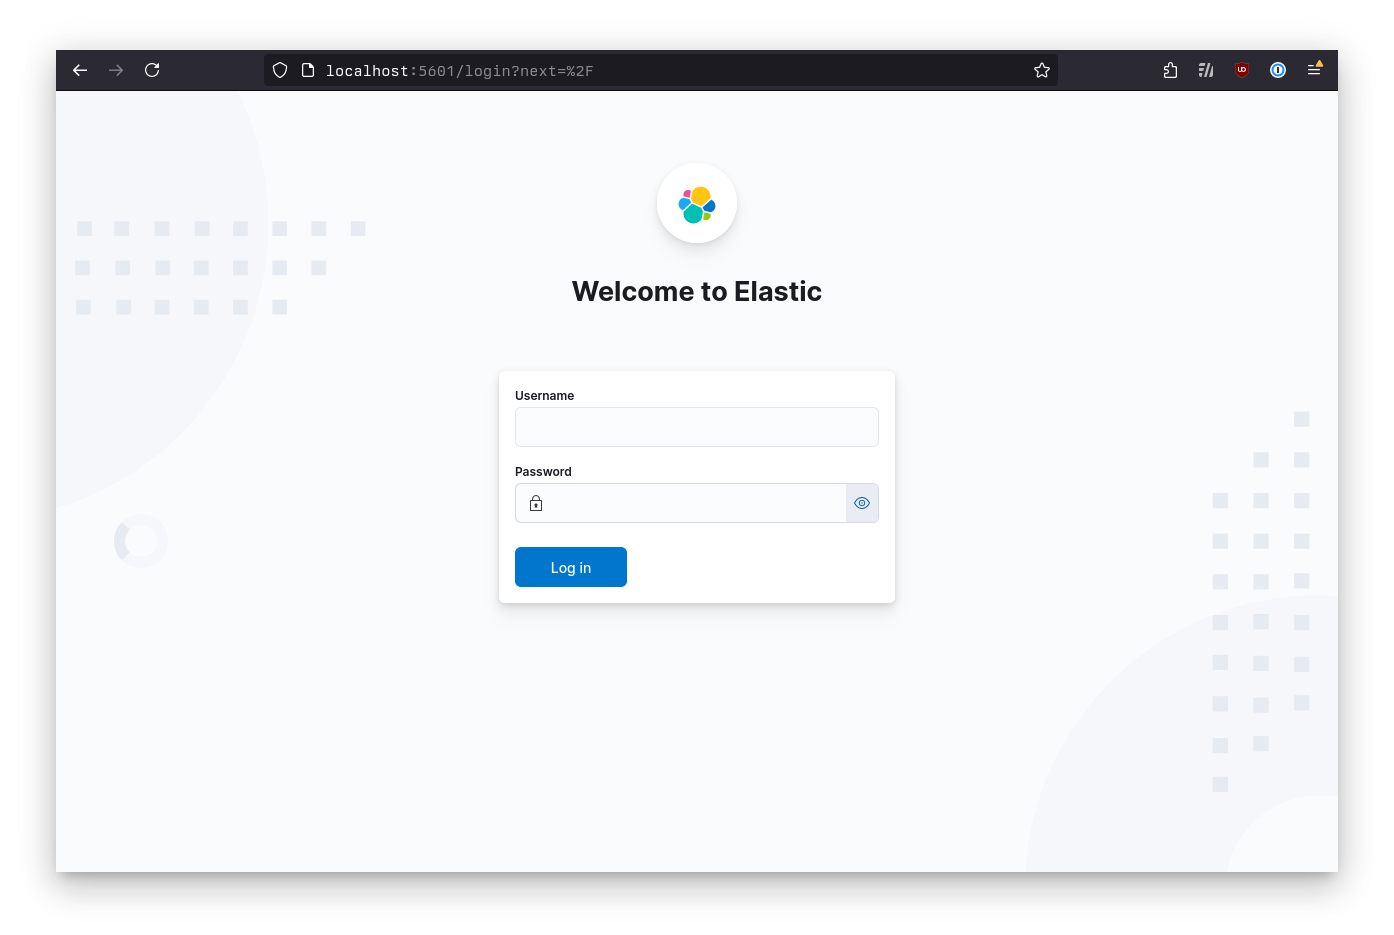
\includegraphics[width=\textwidth]{impl/local1.png}
	\caption{Inicio de sesión en Kibana}
	\label{fig:kibana_login}
\end{figure}

Una vez en la pantalla de inicio de sesión, se puede acceder con las credenciales
definidas en el archivo \texttt{.env} para el usuario \texttt{elastic}.

\begin{figure}[H]
	\centering
	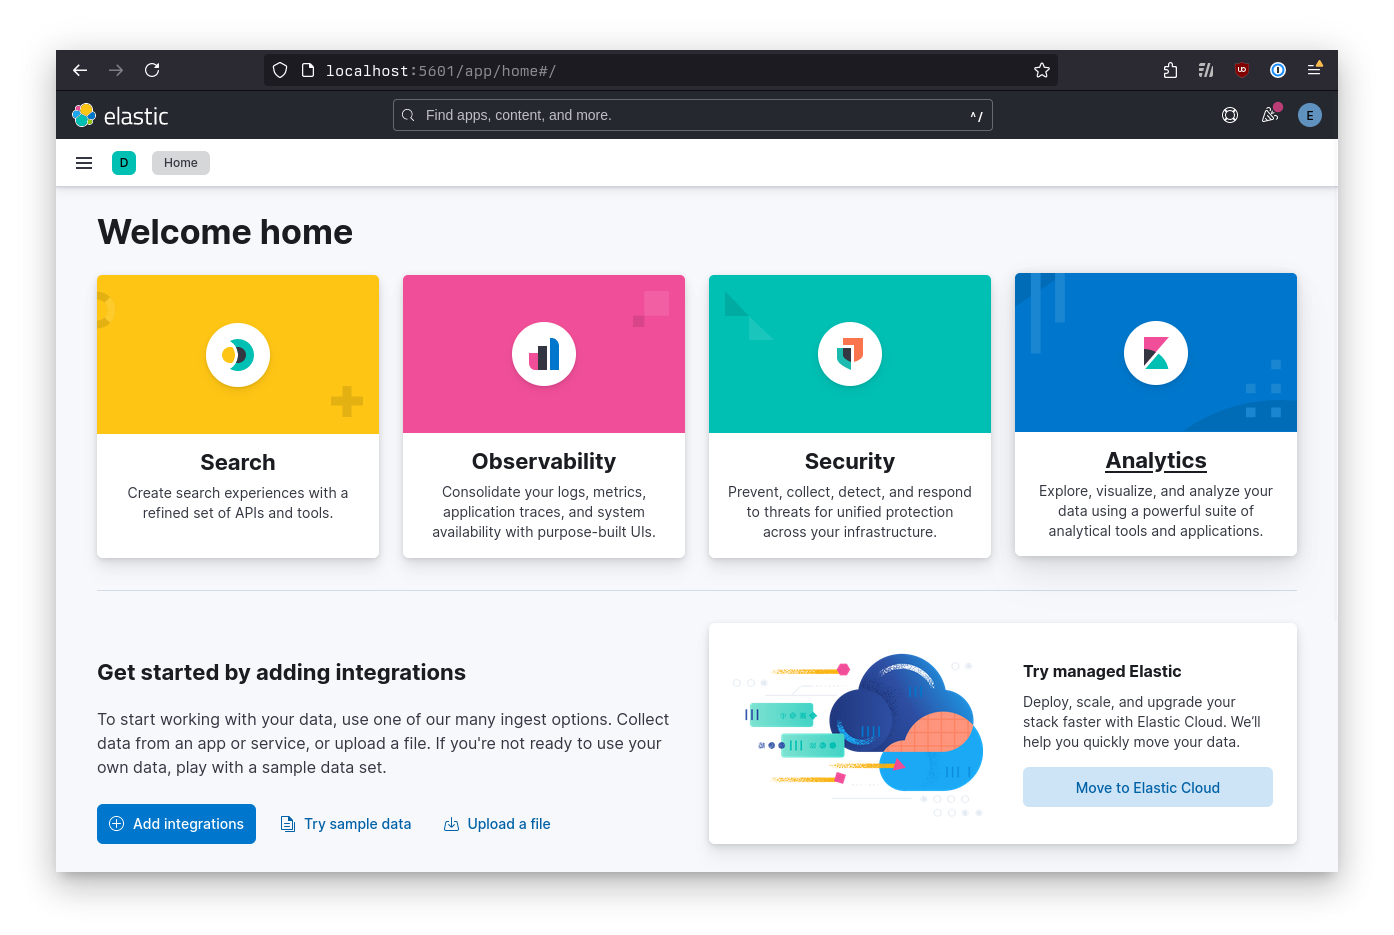
\includegraphics[width=\textwidth]{impl/local2.png}
	\caption{Página de inicio de Kibana}
	\label{fig:kibana_start}
\end{figure}

Una vez aquí, se puede hacer click en la opción \texttt{Try sample data} para
cargar un conjunto de datos de ejemplo y probar la funcionalidad de Kibana con
Elasticsearch. Por supuesto, también se pueden probar la ingesta de datos a
través de Logstash y Kafka o, si así se desea, a través de los \textit{Beats}
especializados de ingesta directa de Elastic.

El manual de uso del sistema se encuentra en \fullref{sec:manual_usuario}.


\newpage{}
\subsection{Proceso de desarrollo}\label{subsec:impl_local_desarrollo}
Para el desarrollo del sistema, se ha seguido un proceso iterativo, comenzando
a partir del ejemplo oficial de Elastic para \textit{Docker Compose}\footnote{
  \url{https://www.elastic.co/blog/getting-started-with-the-elastic-stack-and-docker-compose}
}. A partir de este ejemplo, se añaden progresivamente configuraciones y
servicios, y se prueban las funcionalidades de cada uno de ellos, actualizando
con regularidad el código en el repositorio privado establecido.

\begin{figure}[H]
  \centering
  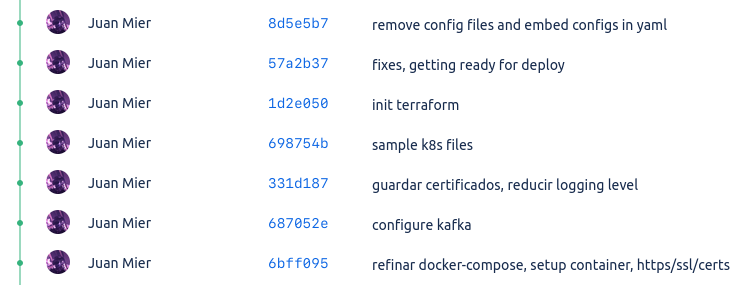
\includegraphics[width=\textwidth]{impl/commits.png}
  \caption{Ejemplo de commits en el repositorio privado}
  \label{fig:commits}
\end{figure}

Inicialmente, se prueban los servicios mínimos (Kibana y Elasticsearch) sin
HTTPS para comprobar su correcto funcionamiento. Una vez se ha comprobado que
los servicios funcionan correctamente, se añade la configuración de seguridad
y se prueban los servicios con HTTPS, ajustando más configuraciones como el
nivel de registro de logs o las comprobaciones de salud de los contenedores.

Una vez se ha comprobado que los servicios funcionan correctamente, se añaden
los servicios de Kafka, Zookeeper y Logstash, y se prueban las conexiones entre
los servicios, ajustando las configuraciones necesarias para que los servicios
se comuniquen correctamente.


\newpage{}
\section{Despliegue \textit{cloud}}\label{sec:impl_cloud}
El desarrollo principal del despliegue en la nube se concentra en la creación
de los scripts de \textit{Terraform} necesarios para la implementación de la
infraestructura planteada en el apartado \fullref{sec:arquitectura}. Para ello,
se divide el proyecto en scripts separados de manera que se puedan gestionar
los recursos y los servicios de manera independiente.

El diseño de una infraestructura base y el desarrollo de un prototipo de manera
local permiten tener una idea clara de los recursos necesarios y de las
características específicas de cada servicio, facilitándo la tarea de
desarrollo.

Para el desarollo, se hace uso de un repositorio privado en \textit{Bitbucket}
para el control de versiones y facilitar a la empresa la revisión y uso del
código. El código completo se encuentra en \fullref{anexo:cloud}.

Esta sección de la memoria documenta el desarrollo de las siguientes historias
de usuario, siguiendo la planificación establecida en la sección \fullref{sec:planif_inicial}:

\begin{table}[H]
	\centering
	\begin{tabular}{|p{0.7\linewidth}|c|c|}
		\hline
		\textbf{Nombre} & \textbf{Prioridad} & \textbf{Tamaño} \\
		\hline
		\hline
		Como desarrollador de Okticket, quiero que la arquitectura se despliegue y orqueste de manera automática & P0\cellcolor{red!50} & XL\cellcolor{red!50} \\
		\hline
  \end{tabular}
  \caption{Lista de HUs cumplimentadas con el despliegue en la nube}
  \label{tab:impl_cloud}
\end{table}


\newpage{}
\subsection{Proceso de desarrollo}\label{subsec:impl_cloud_desarrollo}
El proceso de desarrollo de los scripts de \textit{Terraform} parte de la
implementación original de la infraestructura en local, y se va adaptando a
las necesidades de la infraestructura en la nube, puesto que ambos comparten
similaridades (como la mayoría de la configuración de los servicios, la
estructura general de los mismos, las imágenes y versiones utilizadas, etc.).

Al igual que con el desarrollo local, se sigue un proceso iterativo, comenzando
por la creación de un solo servicio, en este caso Kafka, y continuando con el
resto de la arquitectura. Los primeros despliegues son tan solo pruebas de
concepto, con el objetivo de adaptarse a la infraestructura de la nube, el
funcionamiento de Terraform y la configuración de AWS.

Pese a que Terraform suele encargarse de la creación, modificación y destrucción
de los recursos de manera automática, existen casos en los que es necesaria la
intervención manual, como en la destrucción de los contenedores de
\textit{Secret Manager} o en la actualización de algunas configuraciones de los
recursos. Estos casos ocurrirán solo durante la fase de desarrollo, puesto que
se espera que, en la fase de producción, no sea necesario la reconfiguración de
los recursos y servicios.

La definición de las tareas de ECS durante el desarrollo queda registrado en la
sección correspondiente de AWS, cuyo código y configuraciones se puede consultar
si así se desea.

\begin{figure}[H]
	\centering
	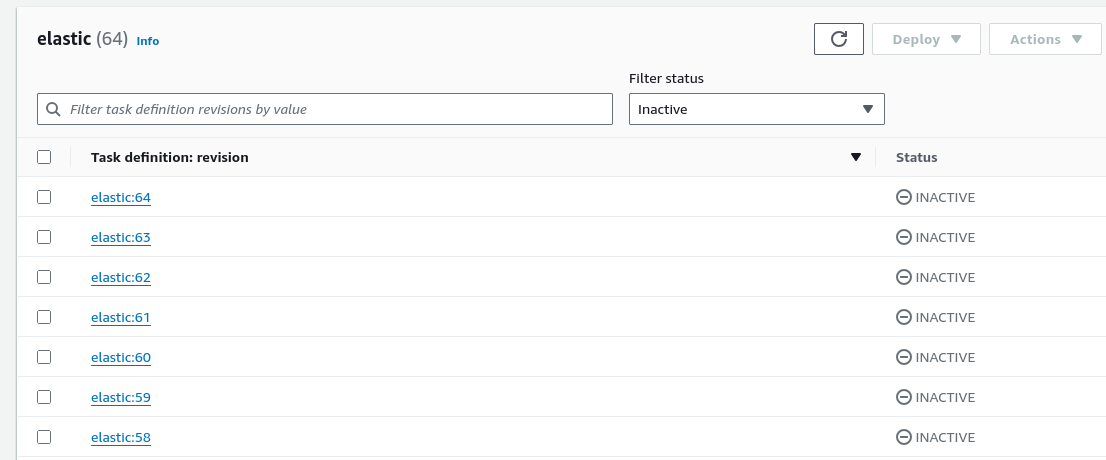
\includegraphics[width=\textwidth]{impl/definitions.png}
	\caption{Ejemplo de definciones de tareas de ECS en AWS}
	\label{fig:definitions}
\end{figure}

\begin{figure}[H]
	\centering
	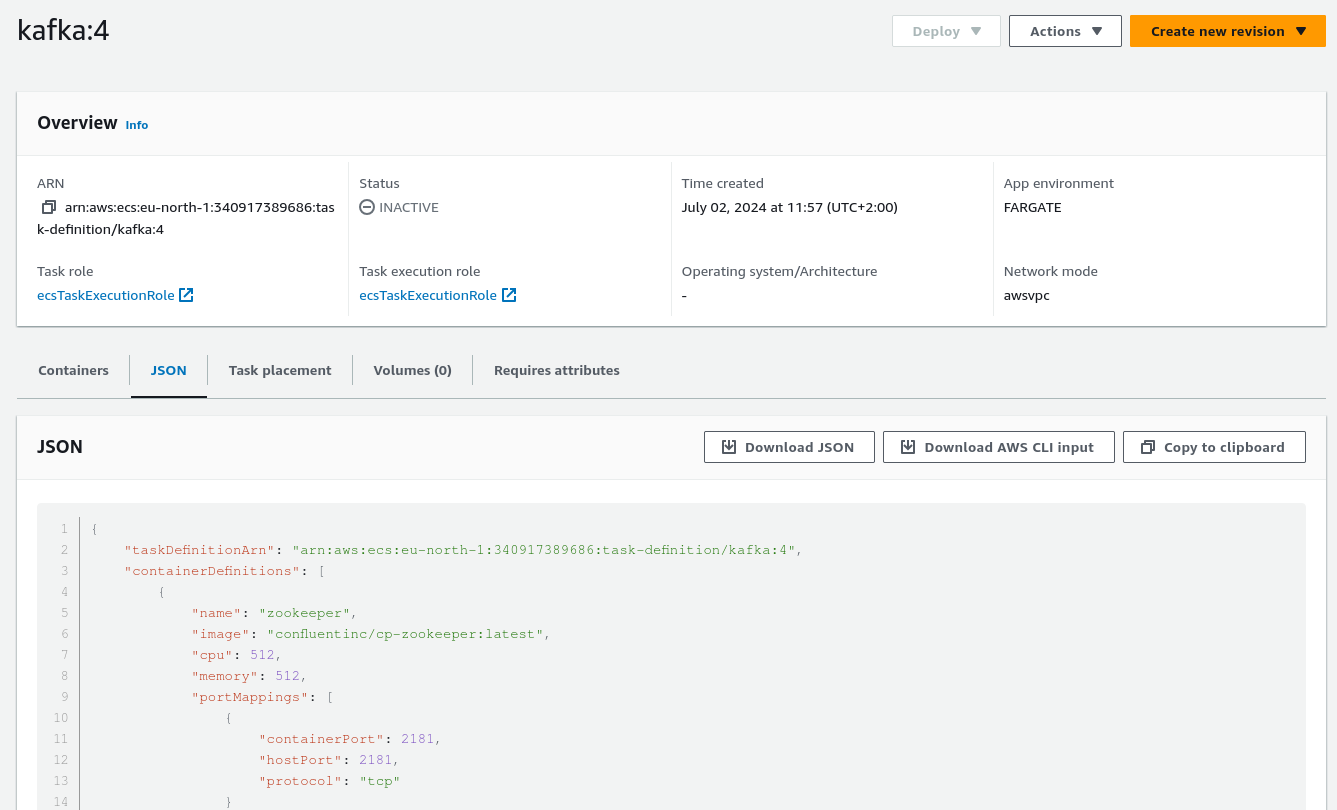
\includegraphics[width=\textwidth]{impl/ejemplo_definition.png}
	\caption{Ejemplo de definción de tarea (Kafka)}
	\label{fig:definition}
\end{figure}


\newpage{}
\subsection{Despliegue de la infraestructura}\label{subsec:impl_cloud_despliegue}
% TODO: desarrollar
% Aquí podría estar bien poner un diagrama de despliegue. Pero que se vea en el
% modelo que ese diagrama de despliegue no es el despliegue de tu proyecto.
% Es decir, el proyecto es crear un proceso de despliegue que hace un despliegue.
% Entonces que se vea que hay ese proceso y luego el diagrama de despliegue de lo
% que el proyecto permite desplegar


\newpage{}
\subsection{Explicación del código}\label{sec:impl_configuracion}
\emph{El código completo se encuentra en el anexo \fullref{anexo:cloud}.}

Los scripts de Terraform se dividen en varios archivos, cada uno de ellos con
una función específica, con el objetivo de facilitar la gestión y configuración
de los recursos y servicios. A continuación, se detallan dichos archivos y su
función en el proyecto.


\subsubsection{Recursos generales}


\subsubsection{Servicios de ELK}


\newpage{}
\section{Ingesta de datos}\label{sec:impl_ingesta}
Tras la creación y el despliegue de la infraestructura base, se procede a la
creación de los scripts de ingesta de datos, de manera escalonada y siguiendo
la prioridad de las fuentes de datos.

Puesto que se ha decidido utilizar Kafka como sistema de mensajería, se
desarrollan los scripts de ingesta de datos para que los datos se envíen a
Kafka y se procesen mediante Logstash y Elasticsearch.

Para la ingesta de datos, se han desarrollado scripts de Python que se encargan
de la lectura de los datos de las fuentes, su transformación y su envío a Kafka.
Estos scripts se ejecutan mediante un \textit{cron} que se encarga de la
ejecución periódica de los mismos.

Esta sección de la memoria documenta el desarrollo de las siguientes historias
de usuario, siguiendo la planificación establecida en la sección \fullref{sec:planif_inicial}:

\begin{table}[H]
	\centering
	\begin{tabular}{|p{0.7\linewidth}|c|c|}
		\hline
		\textbf{Nombre} & \textbf{Prioridad} & \textbf{Tamaño} \\
		\hline
		\hline
		Como desarrollador de Okticket, quiero que se ingesten de manera automática datos de la base de datos interna de MongoDB & P0\cellcolor{red!50} & M\cellcolor{yellow!50} \\
		\hline
		Como desarrollador de Okticket, quiero que se ingesten de manera automática datos de la base de datos interna de MySQL & P0\cellcolor{red!50} & M\cellcolor{yellow!50} \\
		\hline
		Como desarrollador de Okticket, quiero que los datos se limpien de manera automática & P0\cellcolor{red!50} & M\cellcolor{yellow!50} \\
		\hline
		Como desarrollador de Okticket, quiero que se ingesten de manera automática logs de balanceador de AWS & P1\cellcolor{orange!50} & S\cellcolor{green!25} \\
		\hline
  \end{tabular}
  \caption{Lista de HUs cumplimentadas con la ingesta de datos}
  \label{tab:impl_ingesta}
\end{table}



\newpage{}
\section{Visualización de datos}\label{sec:impl_visualizacion}
Una vez se cuentan con datos en Elasticsearch, se puede comenzar el desarrollo
de la visualización de los mismos mediante Kibana. Para ello, se han desarrollado
paneles de visualización que permiten la monitorización de los datos en tiempo
real y la creación de informes y \textit{dashboards} personalizados para cada
modelo de datos contemplado.

Esta sección de la memoria documenta el desarrollo de las siguientes historias
de usuario, siguiendo la planificación establecida en la sección \fullref{sec:planif_inicial}:

\begin{table}[H]
	\centering
	\begin{tabular}{|p{0.7\linewidth}|c|c|}
		\hline
		\textbf{Nombre} & \textbf{Prioridad} & \textbf{Tamaño} \\
		\hline
		\hline
		Como trabajador de Okticket, quiero poder ver y consultar datos internos de la empresa & P1\cellcolor{orange!50} & L\cellcolor{orange!50} \\
		\hline
		Como desarrollador de Okticket, quiero poder ver el estado general de la infraestructura & P1\cellcolor{orange!50} & L\cellcolor{orange!50} \\
		\hline
  \end{tabular}
  \caption{Lista de HUs cumplimentadas con la visualización de datos}
  \label{tab:impl_visualizacion}
\end{table}

|TODO| desarrollar y completar.

